%10kLUTs, 100MHz, 500kB RAM em Xilinx Kintex Ultra scale
%fazer um IP: etapas

This work proposes to develop an IP core capable of encoding the MPEG1/2 Layer II. Due to its complexity, planning the different working phases is essential to both achieve the goal and deliver good results. 

The IP core development will be tracked by a \textit{GitHub} repository, a fork of \textbf{\textit{iob-mp2-e}}. This repository is similar to the original \textit{iob-soc}, containing four submodules: \textbf{\textit{iob-cache}}, a high-performance Verilog cache; \textbf{\textit{iob-picorv32}}, a RISC-V processor; \textbf{\textit{twolame}}, an optimized MP2 encoding software (explained in \textit{Background} section); \textbf{\textit{iob-uart}}, a UART core.\\
In a Linux Operating System, the repository is first cloned, allowing to efficiently implement the \textit{twolame} using the IOb-SoC. Once the project is completed, a pull request is submitted to change the upstream repository.

The work plan is described below, considering \textbf{October 31} as the submission deadline.
Each work phase defines its expected deadline, followed by a brief explanation.


\begin{itemize}
\item \textbf{Emulation on PC} (March 31)\\
This phase consists in emulating the system on PC (\textit{make pc-emul}), which allows easier debugging.

\item \textbf{Profiling} (April 15)\\
This phase consists in analyzing and gaining a better understanding of raw data, by measuring the execution time of the different algorithm parts. This information is useful to understand where the hardware acceleration should be applied (where the bottlenecks are).
%queres real time a 48k samples / s
%stereo

\item \textbf{Hardware implementation} (June 30)\\
This phase consists in the RTL design, which models the digital circuit in terms of the data flow between hardware registers and the logical operations performed. In other words, this phase develops the hardware, which corresponds to the accelerator.
%VHDL Structural Modeling

\item \textbf{Simulation} (July 31)\\
This phase consists in simulating the system, using test benches to exercise and verify the IP core.

\item \textbf{FPGA Synthesis and Implementation} (August 15)\\
This phase consists in compiling and translating the Verilog code into a netlist, followed by the mapping of the synthesized design onto the FPGA.

\item \textbf{Testing} (September 15)\\
This phase consists in testing the system in the FPGA board, allowing evaluation of the IP-core quality and documentation.

\item \textbf{Ethernet} (September 30)\\
This phase consists in implementing the Ethernet standard, which allows hardware communication (transmission of binary data).

\item \textbf{Linting} (October 15)\\
%linting do Verilog
This phase consists in linting the Verilog code. Using a linting tool, the code is checked for programmatic and stylistic errors, in an automated way.

\end{itemize}

Figure \ref{fig:gantt} shows a Gantt chart of the work plan.

\vspace{0.4cm}

\begin{figure}[H]
\centerline{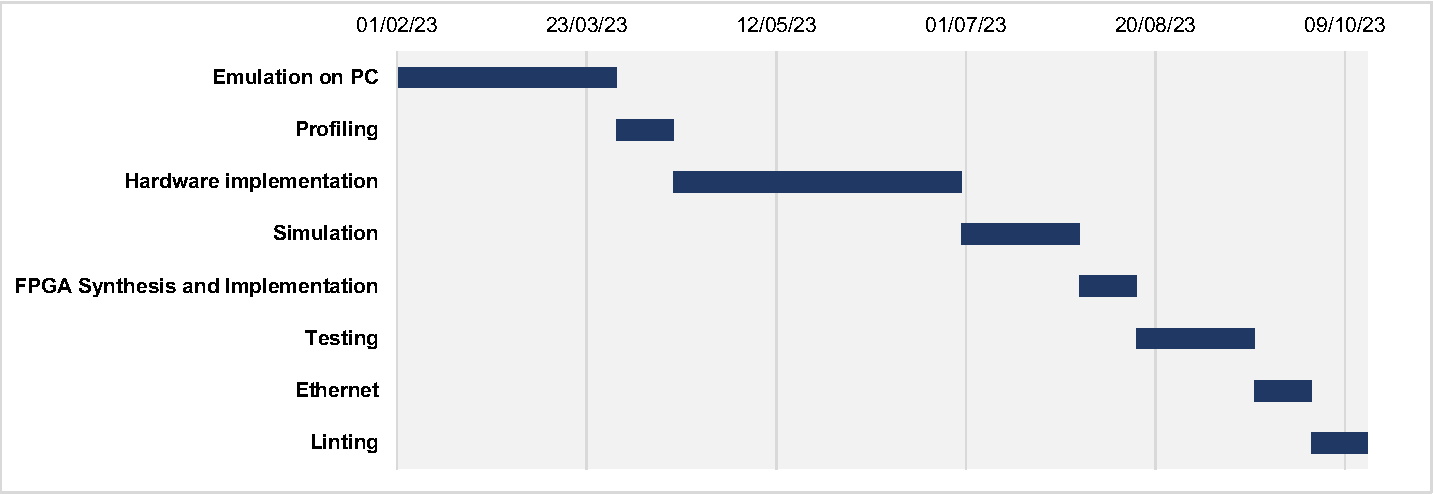
\includegraphics[width=0.99\linewidth]{gantt.pdf}}
\caption{Work plan Gantt chart.}
\label{fig:gantt}
\end{figure}

%avaliaçao de simulation coverage
%(quantas linhas e nós do circuito sao exercitados pela simulação)
%(se nao sao vãop falhar)